\documentclass{article}
\usepackage[utf8]{inputenc}
\usepackage[german]{babel}
\usepackage{graphicx}
\usepackage{amsmath}
\usepackage{booktabs}
\usepackage{hyperref}
\usepackage{listings}
\usepackage{xcolor}
\usepackage{float}
\usepackage[a4paper, margin=1in]{geometry} % Add this line to set the margins


\title{Reinforcement Learning Ansätze für Space Invaders}
\author{Nicola Rohner}
\date{\today}

\begin{document}

\maketitle

\section{Einleitung und Baseline}
Dieser Bericht präsentiert eine systematische Untersuchung verschiedener Reinforcement Learning Varianten für das Atari-Spiel Space Invaders.

\subsection{Baseline-Implementierung}
Die Baseline-Implementierung verwendet eine Random Policy und dient als Referenzpunkt für die Leistungsvergleiche mit den experimentellen Varianten.


\section{Initialer Ansatz}
Der initialer Ansatz konzentriert sich auf die Implementierung von PPO (Proximal Policy Optimization) als Basisalgorithmus

\subsection{Hauptparameter}
\begin{itemize}
    \item Lernrate: 2,5e-4
    \item Anzahl der Schritte pro Update: 128
    \item Anzahl der Minibatches: 4
    \item Anzahl der Optimierungsepochen: 4
    \item Clip-Koeffizient: 0,1
    \item Wertfunktions-Koeffizient: 0,5
    \item Entropie-Koeffizient: 0,01
\end{itemize}

\section{Experimenteller Aufbau}
\subsection{Umgebungskonfiguration}
\begin{itemize}
    \item Gesamtzahl der Zeitschritte: 1.000.000
    \item Anzahl paralleler Umgebungen: 16
    \item Frame Skip: 4 Frames
    \item Beobachtungsraum: 84x84 Graustufenbilder
    \item Frame Stacking: 4 Frames
    \item Aktionsraum: Diskret (Anzahl möglicher Aktionen in Space Invaders)
\end{itemize}

\subsection{Vorverarbeitungspipeline}
\begin{itemize}
    \item NoopReset mit maximal 30 Schritten
    \item Max and Skip Environment Wrapper
    \item Episodic Life Wrapper
    \item Reward Clipping
    \item Graustufenkonvertierung
    \item Frame Stacking
\end{itemize}

\section{Experimentelle Varianten}

\subsection{Variante 1: Hyperparameter-Tuning}
\subsubsection{Motivation}
Das Hyperparameter-Tuning wurde durchgeführt, um den Lernprozess zu optimieren und die Gesamtleistung zu verbessern.

\subsubsection{Modifizierte Parameter}
Die Wahl der optimierten Hyperparameter basiert auf folgenden Überlegungen:
\begin{itemize}
\item \textbf{Learning Rate (0,0005):} Ein leicht erhöhter Wert im Vergleich zur Baseline (0,00025), um die Lerngeschwindigkeit zu verbessern, aber noch niedrig genug, um Stabilität zu gewährleisten.
\item \textbf{Number of Environments (64):} Eine Erhöhung von den ursprünglichen 16 auf 64 parallele Umgebungen. Dies ermöglicht eine bessere Parallelisierung und diversere Erfahrungssammlung. Die grössere Anzahl an parallelen Umgebungen führt zu stabileren Gradienten durch mehr verschiedenartige Samples pro Update.
\item \textbf{Batch Size (4096):} Vergrössert von der ursprünglichen Grösse, um von der erhöhten Anzahl paralleler Umgebungen zu profitieren. Grössere Batches ermöglichen stabilere Gradientenupdates und bessere Ausnutzung der Parallelisierung moderner GPUs. Die Grösse wurde so gewählt, dass sie ein Vielfaches der Anzahl der Umgebungen ist (64 * 64).
\item \textbf{Minibatch Size (1024):} Ein Viertel der Batch Size, was einen guten Kompromiss zwischen Rechneneffizienz und Updatestabilität darstellt. Diese Grösse erlaubt 4 Minibatch-Updates pro Batch, was ausreichend Iterationen für die Optimierung bietet, ohne zu viele Updates durchzuführen, die zu übermässigem Overfitting führen könnten.
\end{itemize}

\subsubsection{Ergebnisse und Analyse}
Die Hyperparameter-Optimierung führte zu konstanter Verbesserung der Performance während des Tranings. Aber nicht sehr signifikant. Wahrscheinlich würde längeres Traning nötig sein, um zu sehen, ob die Verbesserungen wirklich signifikant sind. Die Videos zeigen, dass der Agent das Spiel lernt aber noch nicht wirklich gut darin ist. Es scheint, dass der Agent noch nicht genügend generalisiert hat und noch weiter trainiert werden muss.
Das Ausweichen von Schüssen und klares zielen auf die Invaders ist auch noch nicht zu sehen.
\newpage
\subsection{Variante 2: IMPALA-Architektur}
\subsubsection{Motivation}
Die IMPALA-Architektur wurde implementiert, um die Merkmalsextraktion und Repräsentationslernfähigkeiten durch ihre Residual-Blöcke und tiefere Netzwerkstruktur zu verbessern.

\subsubsection{Implementierungsdetails}
\begin{itemize}
    \item Initiale Kanäle: 16
    \item Drei IMPALA-Blöcke mit Residual-Verbindungen
    \item Merkmalsdimension: 256
    \item MaxPool-Schichten zwischen den Blöcken
\end{itemize}

\begin{figure}[H]
    \centering
    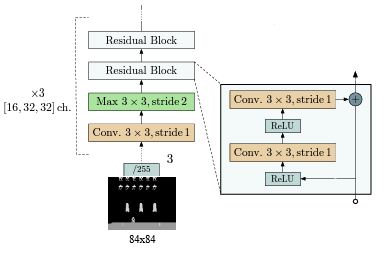
\includegraphics[width=0.8\textwidth]{./Figure_2.png}
    \caption{IMPALA-Blöcke CNN Architektur}
\end{figure}


\subsubsection{Ergebnisse und Analyse}
Diese Erweiterung scheint Verbesserungen zu bringen. Der Agent kann schneller lernen flacht aber gegen Ende der Trainingszeit ab. Die Videos zeigen, dass der Agent das erste Level knapp meistert, jedoch das zweite Level noch nicht wirklich gelernt hat. Dies könnte darauf hindeuten, dass das Modell noch nicht genügend generalisiert hat und noch weiter trainiert werden muss.
\newpage
\subsection{Variante 3: Modifizierter Beobachtungsraum}
\subsubsection{Motivation}
Der Beobachtungsraum wurde modifiziert, um sich auf die relevantesten Teile des Spielbildschirms zu konzentrieren, wodurch potenziell Rauschen reduziert und die Lerneffizienz verbessert wird.

\subsubsection{Implementierungsdetails}
\begin{itemize}
    \item Beschneidung der unteren Hälfte des Bildschirms
    \item Beibehaltung der 84x84 Auflösung nach der Beschneidung
    \item Modifizierte Vorverarbeitungspipeline
\end{itemize}

\begin{figure}[H]
    \centering
    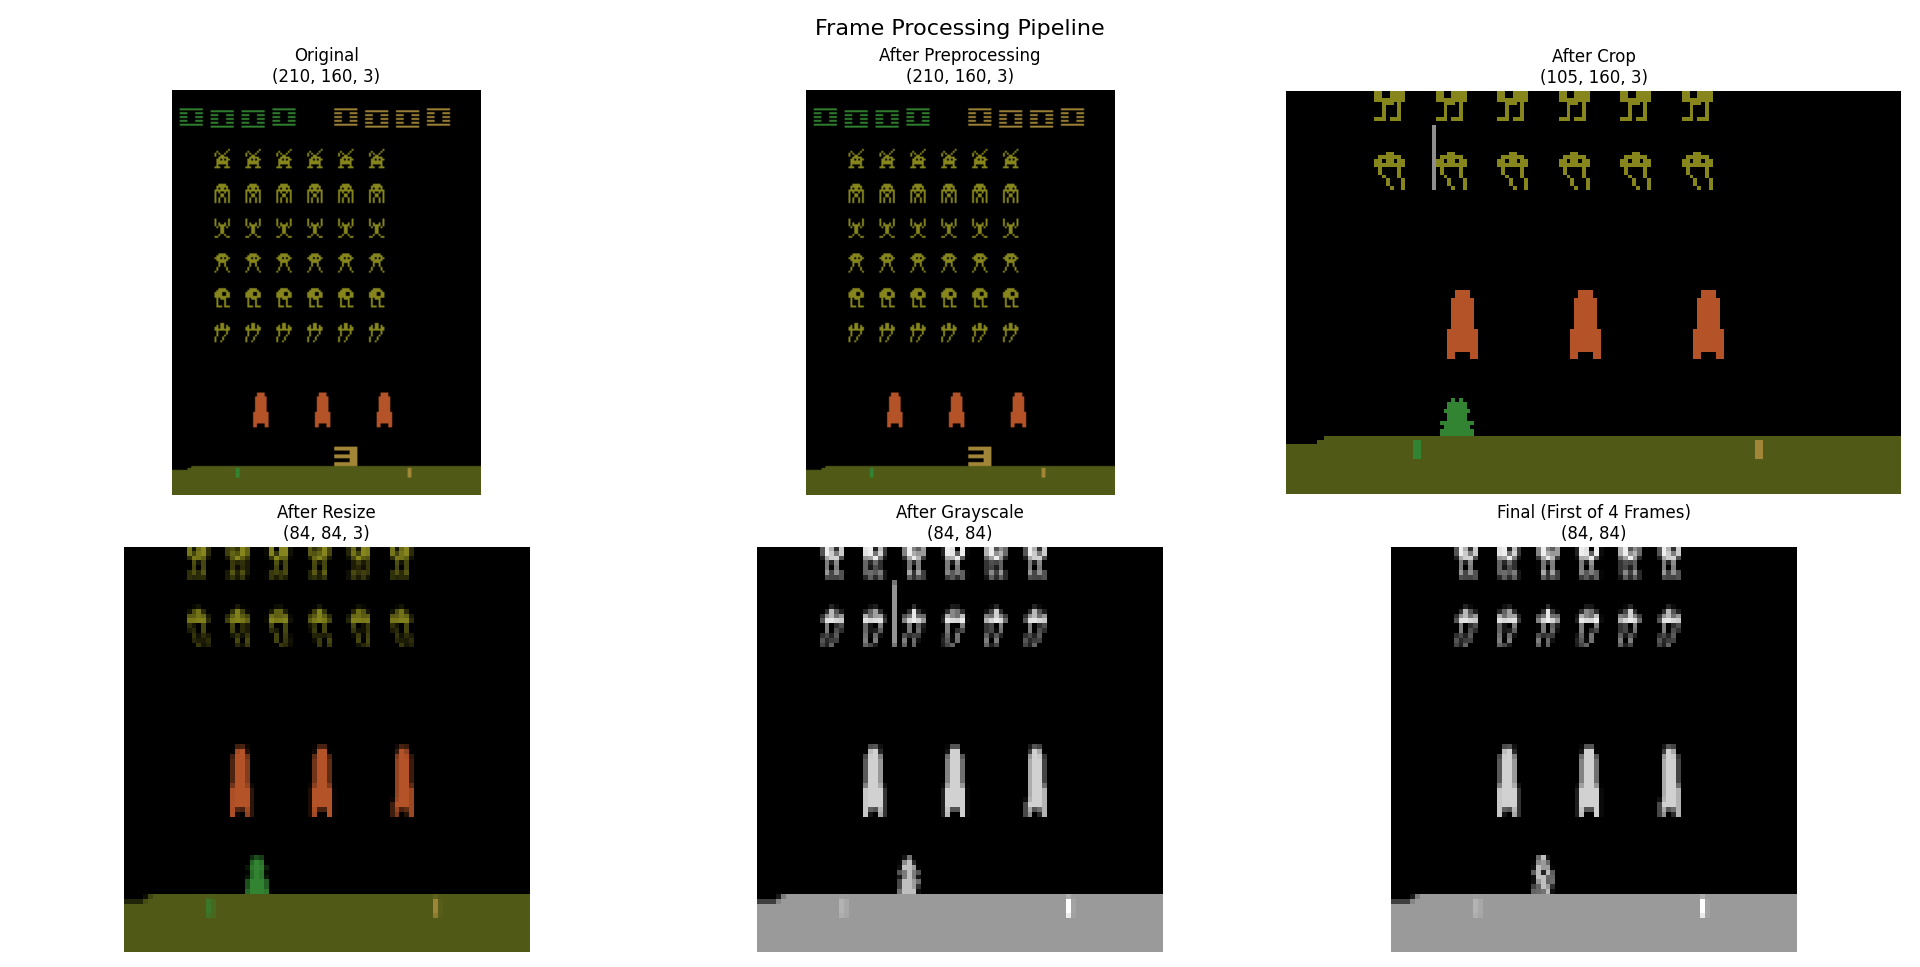
\includegraphics[width=0.8\textwidth]{./Figure_1.png}
    \caption{Prozess der Beobachtungsraum-Modifikation}
\end{figure}


\subsubsection{Ergebnisse und Analyse}
Während des Tranigns sieht man eine leicht erhöhten Return und Episodic Length. Jedoch ist die Verbesserung nicht so gross wie erwartet. Dies könnte daran liegen, dass die untere Hälfte des Bildschirms nicht so relevant ist, wie angenommen. Eine weitere Untersuchung wäre nötig, um zu sehen, ob die Modifikation des Beobachtungsraums wirklich einen Einfluss auf das Lernverhalten des Agenten hat.
In den Videos sieht man auch nicht wirklich ein klarer Fokus auf die unteren Invaders, was darauf hindeutet, dass der Agent nicht wirklich lernt, dass die unteren Invaders auch relevant sind.
Eventuell müsste man das Reward-System anpassen. Denn wenn der Agent Inavders ausserhalbt des Fokus abschiesst, wird er trotzdem belohnt. Dies könnte dazu führen, dass der Agent nicht lernt, dass es wichtig ist, die Invaders im Fokus zu halten.

\newpage
\subsection{Variante 4: Survival Time Bonus}
\subsubsection{Motivation}
Ein zentrales Problem beim Training von Agenten in Space Invaders ist die Tendenz zu riskanten Strategien, die zwar kurzfristig hohe Punktzahlen erzielen können, aber zu vorzeitigem Spielende führen. Um dieses Problem anzugehen, wurde ein Überlebenszeitbonus eingeführt, der längeres Überleben belohnt und damit indirekt defensive Strategien fördert.

\subsubsection{Implementierungsdetails}
\begin{itemize}
    \item Einführung eines konstanten Überlebenszeitbonus von 1 pro Zeitschritt
    \item Integration nach dem ClipRewardEnv-Wrapper in der Vorverarbeitungspipeline
    \item Bonus wird nur in nicht-terminalen Zuständen angewendet
\end{itemize}

Der Überlebenszeitbonus wurde bewusst grösser gewählt, um den Einfluss dieser Änderung auf das Lernverhalten des Agenten zu verstärlken.


\subsubsection{Ergebnisse und Analyse}
Die Integration des Überlebenszeitbonus führte zu folgenden Beobachtungen:
\begin{itemize}
    \item Verlängerung der durchschnittlichen Episodendauer
    \item Deffensivere Spielstrategien, Agent bleibt of auf der Linken Seite
    \item Durchschnittlich kleinere Punktzahlen, aber insgesamt höhere Überlebenszeit
\end{itemize}


\newpage

\section{Vergleichende Analyse}
\begin{figure}[H]
    \centering
    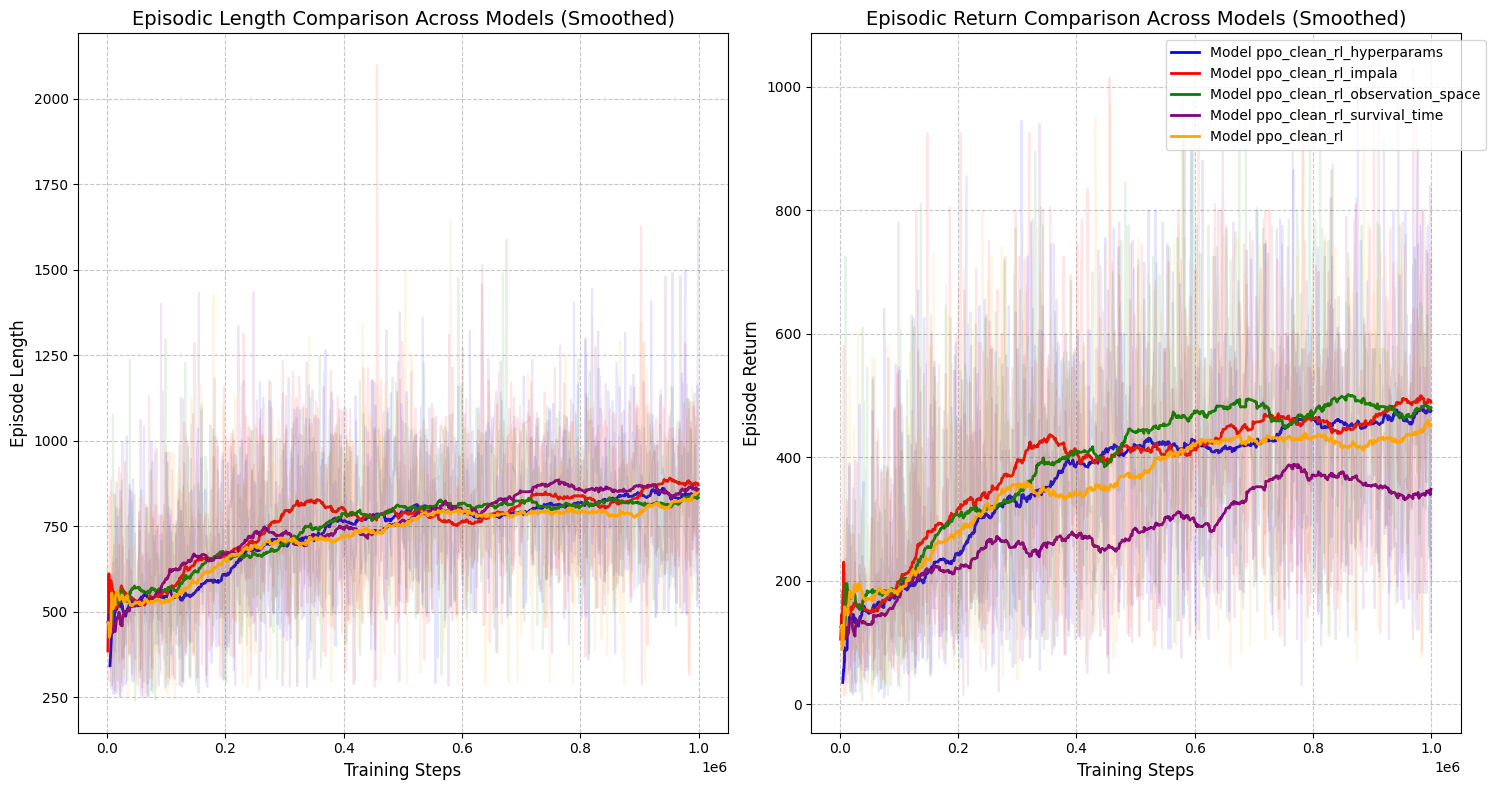
\includegraphics[width=0.8\textwidth]{./Figure_3.png}
    \caption{Vergleiche von return und episode length während des Trainings}
\end{figure}

Evaluation für 100 Episoden

\begin{tabular}{lrrrr}
\toprule
Variante & Mean Return & Standardabw. & Min. Return & Max. Return \\
\midrule
Baseline Random & 2.7 & 3.7 & 0 & 28 \\
Initial PPO & 493.45 & 174.2 & 70 & 1080 \\
Hyperparameter Optimiert & 471.7 & 149 & 85 & 800 \\
IMPALA Architektur & 476.15 & 164.8 & 145 & 940 \\
Modifizierter Beobachtungsraum & 461 & 136 & 125 & 765 \\
Survival Time Bonus & 352.4 & 163.2 & 110 & 805 \\
\bottomrule
\end{tabular}

\section{Fazit \& Ausblick}

Die Evaluation zeigt das die Varianten gegenüber Random Baseline eine Verbesserung darstellen. Gegnüber originallen PPO-Modell sind die Verbesserungen jedoch nicht so gross.
Spannenede Beobachtungen sind das IMPALA und Modifizierten Beobachtungsraum Verbesserungen bei min Return zeigen aber nicht Max Return.
Zudem scheint der Survival Time Bonus eine defensive Spielstrategie zu fördern, was zu einer längeren Überlebenszeit führt, aber zu kleineren Punktzahlen.
\newline

Generell würde ich die einzelnen Erweiterungen kombinieren und testen, ob sich die Leistung weiter verbessert. 
Zudem würde ich die Modelle länger tranieren lassen um zu sehen ob sich die Varianz der Ergebnisse verringert und die Modelle stabiler werden. Momentan ist noch nicht ein wirkliches Plateau erreicht, was darauf hindeutet, dass die Modelle noch nicht vollständig konvergiert sind.
Auch die Video zeigen das erste Level gut gemeistert wird, jedoch das zweite Level noch nicht wirklich gelernt wurde.
Wenn ein Plateau erreicht ist, würde ich mir die Videos anschaun und versuchen zu verstehen wo das Modell noch Schwächen hat. Daraus würde ich dann Handlungsempfehlungen ableiten, um das Modell weiter zu verbessern.
Wie z.B das Reward-System anpassen: Reward abschwächen für Misses oder Hits, die nicht zu einem Abschuss führen. In der Hoffnung, dass der Agent dann nicht mehr so viele Schüsse abfeuert, die nicht zielführend sind.






\end{document}